\documentclass[sigplan,anonymous,review,screen]{acmart}

%% ACM bibliographic strip cleanup for an anonymous draft.
\setcopyright{none}
\acmConference[CPP '27]{Certified Programs and Proofs}{January 2027}{Mexico City, Mexico}
\acmYear{2027}
\acmISBN{}
\acmDOI{}
\settopmatter{printacmref=false,printccs=false,printfolios=true}

\usepackage{mathtools}
\usepackage{amsthm}
\usepackage{amssymb}
\usepackage{hyperref}
\usepackage{cleveref}
\usepackage{listings}
\usepackage{xcolor}
\usepackage{tikz}
\usetikzlibrary{positioning,arrows.meta,calc}

%% cleveref names for listings (default cleveref does not know about
%% the listings package's `lstlisting' counter).
\crefname{lstlisting}{Listing}{Listings}
\Crefname{lstlisting}{Listing}{Listings}

%% Two-column body has long \texttt{} module names that the line breaker
%% cannot split (e.g. `Rademacher.FiniteSampleSymmetrization'). Allow
%% extra stretch on the last paragraph pass before declaring overfull.
%% Inline insertions of \allowbreak between dotted segments handle the
%% worst offenders.
\setlength{\emergencystretch}{3.5em}

%% Lean 4 listing style.
\definecolor{leanbg}{rgb}{0.97,0.97,0.97}
\definecolor{leankw}{rgb}{0.10,0.10,0.55}
\definecolor{leanco}{rgb}{0.30,0.50,0.30}
\definecolor{leanst}{rgb}{0.55,0.20,0.20}
\lstdefinelanguage{Lean4}{
  morekeywords={theorem,lemma,def,noncomputable,variable,namespace,end,open,
                section,by,fun,let,in,if,then,else,match,with,do,return,
                instance,class,structure,inductive,where,abbrev,Type,Prop,
                Sort,have,show,exact,intro,intros,apply,refine,calc,using,
                this,rfl,trivial},
  morecomment=[l]{--},
  morecomment=[s]{/-}{-/},
  morestring=[b]",
  sensitive=true,
}
\lstset{
  language=Lean4,
  basicstyle=\ttfamily\footnotesize,
  keywordstyle=\color{leankw}\bfseries,
  commentstyle=\color{leanco}\itshape,
  stringstyle=\color{leanst},
  backgroundcolor=\color{leanbg},
  frame=single,
  framesep=3pt,
  rulecolor=\color{leanbg},
  showstringspaces=false,
  breaklines=true,
  columns=fullflexible,
  keepspaces=true,
  xleftmargin=4pt,
  xrightmargin=2pt,
  aboveskip=6pt,
  belowskip=6pt,
}

%% Math shortcuts.
\newcommand{\Risk}{\mathcal{R}}
\newcommand{\eRisk}{\widehat{\mathcal{R}}}
\newcommand{\Rad}{\widehat{\mathfrak{R}}}
\newcommand{\KL}{\mathrm{KL}}
\newcommand{\E}{\mathbb{E}}
\newcommand{\Prob}{\mathbb{P}}
\newcommand{\R}{\mathbb{R}}
\newcommand{\N}{\mathbb{N}}
\newcommand{\Hyp}{\mathcal{H}}
\DeclareMathOperator*{\argmin}{arg\,min}
\DeclareMathOperator*{\esssup}{ess\,sup}

\begin{document}

\title{A Finite-First Spine for Statistical Learning Theory: Machine-Checked PAC-VC Bounds in Lean 4}

\author{Anonymous Author(s)}
\affiliation{%
  \institution{Institution Withheld for Review}
  \country{}
}
\email{anon@example.com}

\renewcommand{\shortauthors}{Anonymous}

\begin{abstract}
We present FormalSLT, a Lean 4 library that formalizes the classical
pedagogical route through statistical learning theory --- empirical risk
minimization, Rademacher symmetrization, Massart's finite-class bound,
the Sauer--Shelah polynomial growth bound, the binary VC bridge, an
Azuma-route generalization-gap tail, and a VC ERM excess-risk
guarantee --- as a connected chain of machine-checked theorems with
explicit constants. The library extends the spine with a Ledoux--Talagrand
contraction lemma, a Rademacher bound for finite-dimensional linear
predictor classes, finite multiscale Dudley-style entropy-budget
wrappers, an algorithmic-stability bounded-differences scaffold in the
sense of Bousquet and Elisseeff, and a PAC-Bayes change-of-measure
foundation comprising the finite KL divergence, the Donsker--Varadhan
variational inequality, and a finite iid product moment-generating
function bridge, plus a closed Catoni-form high-confidence payoff and
finite-grid McAllester-style wrappers for $[0,1]$ losses. We adopt a
deliberate \emph{finite-first} methodology:
hypothesis classes are finite index types, samples are coordinates of a
product measure, and the Dudley layer is a discrete entropy-budget
wrapper extended by total-bounded finite-net and supplied-supremum boundary
adapters rather than a continuous integral. Forty-five Lean modules and
19,339 lines of proof are checked against
Mathlib4 with no \texttt{sorry}, no \texttt{admit}, and no custom axioms;
the public theorem spine reduces to the canonical Lean axiom set
$\{\texttt{propext},\,\texttt{Classical.choice},\,\texttt{Quot.sound}\}$.
The contribution is complementary to recent work on continuous
empirical-process theory in Lean 4, which targets continuous Dudley,
log-Sobolev, Efron--Stein, Gaussian Poincar\'e, and minimax rates: the
two efforts cover disjoint theorem families and can be used jointly.
The library is publicly available; a commit-pinned artifact accompanies
the submission.
\end{abstract}

\keywords{statistical learning theory, formal verification, Lean 4,
Mathlib, VC dimension, Rademacher complexity, PAC-Bayes, algorithmic
stability}

\maketitle

\section{Introduction}
\label{sec:intro}

Statistical learning theory provides the mathematical guarantees behind
modern machine learning: when a classifier or regressor selected on a
training sample will, and will not, generalize to new data drawn from
the same distribution. The canonical results --- the
Vapnik--Chervonenkis polynomial growth bound on shatter coefficients,
Massart's finite-class Rademacher bound, McDiarmid's bounded-differences
inequality, the symmetrization argument that connects empirical and
ghost samples, Bousquet and Elisseeff's stability theorems for
algorithmic generalization, and the PAC-Bayes change-of-measure
inequalities of McAllester, Seeger, and Catoni --- chain together so
that a single weakened hypothesis can invalidate constants several
pages downstream. The proofs are short on paper but their hypotheses
and constants are easy to blur in informal writing. The 1989 paper of Blumer,
Ehrenfeucht, Haussler, and Warmuth on VC-based learnability
\cite{Blumer1989} is the canonical reference for the
PAC framework, and its careful treatment of separability and
measurability assumptions was already a corrective to less guarded
treatments. Subsequent textbook expositions
\cite{ShalevShwartz2014, BoucheronLugosiMassart2013}
trade away some of that care for pedagogical accessibility, leaving the
reader to reconstruct exactly which hypothesis class shape, which
boundedness assumption, and which constant is in force at each step.

This paper contributes \emph{FormalSLT}, a Lean 4 library that turns
the standard pedagogical route from empirical risk minimization to the
VC ERM excess-risk tail into a connected chain of machine-checked
theorems, and adds three further tracks --- contraction, finite chaining
budgets, and PAC-Bayes / stability foundations --- to the same spine.
The library is built on top of Mathlib4 and contains no \texttt{sorry},
no \texttt{admit}, and no custom axioms; every public theorem reduces
to the canonical axiom set $\{\texttt{propext},
\texttt{Classical.choice}, \texttt{Quot.sound}\}$ that the wider
Mathlib community has standardized on.

The defining methodological choice is what we call the
\emph{finite-first} approach. Hypothesis classes are finite index types
$\iota$ with $[\texttt{Fintype}\;\iota]$, samples are functions
$\texttt{Fin}\,n \to Z$ drawn from a product measure on a measurable
space, suprema over the hypothesis class are finite maxima, and the
Dudley layer is a finite multiscale entropy-budget wrapper rather than
a continuous integral. The choice is deliberate. Finite hypothesis
classes are where ML practice lives: every neural network deployed in
production is, at floating-point resolution, a finite class; every
tree-based learner has a finite (if astronomically large) hypothesis
space; every implementation of regularization carves out a finite,
discrete predictor family. The combinatorial structure that drives the
finite-class bounds --- Sauer--Shelah polynomial growth, the
log-cardinality factor in Massart, the dyadic chaining envelope of
Dudley --- is sharper and more readable in the finite setting than its
continuous analogue, and the formalization avoids the measurability,
separability, and $\sigma$-algebra hygiene that dominate continuous
empirical-process arguments.

The finite-first choice is not an attempt to replace the continuous
theory. A contemporaneous Lean 4 effort, YuanheZ et~al.\
\cite{YuanheZ2026}, formalizes the continuous Dudley entropy
integral, Gaussian Lipschitz concentration, the bounded-difference
inequality via log-Sobolev, the Gaussian Poincar\'e and Efron--Stein
inequalities, sparse least-squares regression with sharp rates, and
small-ball / minimax tooling. Their library is the natural home for the
continuous track. Our library covers the disjoint finite-first PAC-VC
track plus contraction, linear predictors, stability scaffolding, and
PAC-Bayes change of measure. The two libraries can be used jointly in
downstream developments.

\Cref{sec:background} sketches the statistical learning theory
background and the Lean 4 conventions we rely on.
\Cref{sec:related} positions FormalSLT against contemporaneous Lean,
Coq, and Isabelle work. \Cref{sec:library} is the technical
core: the architecture, the PAC-VC spine, the PAC-Bayes track, and the
algorithmic-stability track. \Cref{sec:engineering} discusses the
proof-engineering decisions that shaped the library and documents the
boundaries we have not yet crossed. \Cref{sec:conclusion}
sketches the next theorem targets and the relationship to upstream
Mathlib.

\section{Background}
\label{sec:background}

The statistical learning setting fixes a measurable space $Z$ of
labeled examples, a probability measure $\mu$ on $Z$, a finite index
type $\iota$ for the hypothesis class, and a real-valued loss
$\ell : \iota \to Z \to \R$. The two principal quantities are the
\emph{population risk} $\Risk(i) = \int \ell(i, z)\,d\mu(z)$ and the
\emph{empirical risk}
$\eRisk_S(i) = n^{-1} \sum_{k=1}^{n} \ell(i, S_k)$ on an iid sample
$S \sim \mu^{\otimes n}$. The \emph{generalization gap}
$\Risk(i) - \eRisk_S(i)$ measures how much the empirical estimate
underestimates the population risk; the supremum of this gap over the
hypothesis class is the relevant quantity to control because empirical
risk minimization selects $i$ adversarially with respect to it.

The Rademacher complexity of a class $F$ on a sample $S$ is
$\Rad_S(F) = \E_\sigma \sup_{f \in F} n^{-1} \sum_k \sigma_k\, f(S_k)$,
where $\sigma$ is a uniform sign vector on $\{-1, +1\}^n$. The two
classical decompositions of the generalization gap are the
symmetrization inequality
$\E_S \sup_i (\Risk(i) - \eRisk_S(i)) \le 2\, \E_S \Rad_S(\ell \circ \Hyp)$
and the bounded-differences inequality, which yields a sub-Gaussian tail
on the deviation of the gap from its expectation by way of either
Azuma's martingale inequality or McDiarmid's product-kernel
decomposition.

A class $\Hyp$ of binary classifiers $h : \mathcal{X} \to \{0, 1\}$
shatters a finite set $A \subseteq \mathcal{X}$ if every binary pattern
on $A$ is realized by some $h \in \Hyp$. The
Vapnik--Chervonenkis dimension of $\Hyp$ is the largest $d$ such that
some $A$ of cardinality $d$ is shattered, and the Sauer--Shelah lemma
bounds the number of distinct binary patterns realized on any
$n$-point sample by $\sum_{k=0}^{d} \binom{n}{k} \le (en/d)^d$. A
parallel notion of \emph{effective class} replaces binary patterns with
loss patterns: two hypotheses are equivalent on $S$ if they induce the
same vector $(\ell(i, S_1), \ldots, \ell(i, S_n))$. For binary
classifiers under 0/1 loss the two notions coincide.

The PAC-Bayes framework lifts the analysis from a single hypothesis to
a posterior distribution $\rho$ over $\iota$, controlled by a prior
$\pi$ that is fixed before seeing data. The key change-of-measure
inequality is Donsker--Varadhan's variational identity,
$\sum_i \rho_i\, f_i \le \KL(\rho \,\|\, \pi)
                       + \log \sum_i \pi_i\, e^{f_i}$,
which, applied to the centered empirical-risk deviation
$f_i = \lambda(\Risk(i) - \eRisk_S(i))$ and combined with a moment
generating function bound and Markov's inequality, yields the
McAllester confidence bound on the posterior generalization gap.
Algorithmic stability replaces uniform-convergence reasoning with a
sensitivity analysis of the learning algorithm $A : Z^n \to \iota$:
if replacing a single training example shifts the loss of $A(S)$ by at
most $\beta$ on every test point (uniform stability), then the
expected generalization gap is bounded by $\beta$ and a
bounded-differences argument turns this into a high-probability
bound \cite{BousquetElisseeff2002}.

Lean 4 \cite{deMoura2021} is a dependent-type-theoretic proof
assistant whose mathematics library Mathlib4
\cite{Mathlib2020} provides the measure-theoretic, topological,
and order-theoretic infrastructure on which we build. Three
foundational axioms underpin classical mathematics in Lean: propositional
extensionality (\texttt{propext}), the axiom of choice
(\texttt{Classical.choice}), and the soundness of quotient types
(\texttt{Quot.sound}). The Mathlib community has standardized on this
trio, and any Lean theorem whose \texttt{\#print axioms} output reduces
to it is accepted as ``classically axiomatic'' without further hidden
assumptions. The discipline of avoiding \texttt{sorry} placeholders,
\texttt{admit} markers, and ad-hoc \texttt{axiom} declarations is a
hard requirement of the artifact: every theorem cited in this paper
satisfies it, verified by an axiom audit
that runs against a pinned commit and accompanies the artifact.

\section{Related Work}
\label{sec:related}

\paragraph{Lean 4 / Mathlib formalizations of learning theory.}
The closest contemporary to this work is the Lean 4 library of
YuanheZ et~al.\ \cite{YuanheZ2026}, \emph{Statistical Learning
Theory in Lean 4: Empirical Processes from Scratch}, which targets the
continuous empirical-process route: continuous Dudley entropy
integrals for sub-Gaussian processes, Gaussian Lipschitz concentration,
the Bernoulli log-Sobolev inequality, Efron--Stein, Gaussian
Poincar\'e, Han's inequality, entropy duality and subadditivity,
covering-number theory, sparse least-squares regression with sharp
rates, small-ball methods, and minimax lower bounds. Their library is
substantially larger ($\sim$30k lines) and is intended as a research
formalization substrate for empirical-process theory. The two efforts
are complementary: their published results table does not include
Sauer--Shelah polynomial growth, an ERM excess-risk tail, the binary VC
bridge, the Ledoux--Talagrand contraction lemma, a finite-dimensional
linear-predictor Rademacher bound, an algorithmic-stability scaffold,
or a PAC-Bayes Donsker--Varadhan layer. We do not formalize the
continuous Dudley integral, the log-Sobolev / Efron--Stein / Poincar\'e
functional inequalities, sparse-regression rates, or minimax lower
bounds. A reader who needs both directions can compose the libraries
as Lean dependencies.

A second Lean 4 effort, MohanadAhmed \cite{MohanadAhmed2025}, formalizes
the symmetrization inequality, McDiarmid's bounded-differences
inequality, and Hoeffding's lemma, with later versions reaching toward
Dudley's entropy integral. The overlap with our library is the
Rademacher symmetrization step itself; we extend the spine through
Massart, the Sauer--Shelah polynomial bound, the binary VC bridge, and
the VC ERM excess-risk tail, none of which appear in MohanadAhmed.

The earliest machine-checked PAC-learnability theorem we are aware of
is the Lean 3 / Mathlib3 development of Tassarotti, Vajjha, Banerjee,
and Tristan at CPP 2021 \cite{Tassarotti2021}, who formalize the full
measure-theoretic PAC learnability of the decision-stump class on the
real line. Their proof carefully separates deterministic combinatorial
reasoning from probabilistic reasoning over a fixed measurable space.
The architectural lesson --- to factor every theorem into a deterministic
core and a probabilistic envelope --- directly informed our split between
the finite-sample sign-vector core (\texttt{Rademacher.FiniteSample},
\texttt{Rademacher.FiniteSampleSymmetrization}) and the
product-measure envelope (\texttt{Rademacher.Symmetrization},
\texttt{Rademacher.HighProbability}). Their work is the only prior
formal PAC learnability result for a specific class; ours formalizes
the abstract finite-class machinery one layer higher.

\paragraph{Coq formalizations.}
Bagnall and Stewart's MLCERT system \cite{BagnallStewart2019} is the
closest Coq counterpart: a finite-hypothesis-class PAC bound via
Hoeffding and a union bound, with extraction to executable learning
procedures certifying their generalization. Their proof uses the
two-step Hoeffding-plus-union route, which yields a $\log|\Hyp|$ rate
that does not adapt to effective class size. Our route through
Rademacher symmetrization, Massart, and Sauer--Shelah is the longer
six-stage pipeline that gives the standard $O(\sqrt{d \log(n/d)/n})$
rate when the VC dimension $d$ is much smaller than $\log|\Hyp|$.

\paragraph{Isabelle / HOL formalizations.}
Karayel and Tan's \emph{Concentration Inequalities} entry in the Archive
of Formal Proofs \cite{KarayelTan2023} formalizes Markov, Chebyshev,
Chernoff, Bennett, Bernstein, Bienaym\'e, Cantelli, Efron--Stein,
McDiarmid, and Paley--Zygmund inequalities in Isabelle/HOL. Their
McDiarmid bound is sharper than ours: their constant is the textbook
$2B^2$, whereas our Azuma-route exponent is $8B^2$
(\Cref{sec:engineering}). The Isabelle development is concentration
tooling and does not connect to PAC, VC, or Rademacher complexity.
Bentkamp, Blanchette, and Klakow \cite{Bentkamp2019} formalize a deep
network expressiveness theorem in Isabelle/HOL; the scope is
representation theory rather than generalization.

\paragraph{Verification of ML systems.}
A separate body of work --- including CertRL's verified value- and
policy-iteration convergence proofs in Coq, the FARNN line on neural
network robustness, and various model-checked safety properties of
deep networks --- formalizes properties of \emph{implementations} rather
than the underlying generalization theory. We mention this category to
preempt referee confusion: FormalSLT does not verify a particular
training procedure or neural-network implementation; it formalizes the
mathematical sample-complexity and concentration theorems that any such
verification would invoke.

\paragraph{Mathematical sources we formalize.}
The textbooks and papers we treat as source material for the
\emph{informal} statements are
Vapnik and Chervonenkis~\cite{VapnikChervonenkis1971} for the
combinatorial dimension; Sauer~\cite{Sauer1972} and
Shelah~\cite{Shelah1972} for the polynomial bound on shatter
coefficients; Bartlett and Mendelson \cite{BartlettMendelson2002} for
Rademacher and Gaussian complexities;
Shalev-Shwartz and Ben-David \cite{ShalevShwartz2014} for the
ERM-to-VC pedagogical route;
Bousquet and Elisseeff \cite{BousquetElisseeff2002} for algorithmic
stability; McAllester \cite{McAllester1999}, Seeger
\cite{Seeger2002}, and Catoni \cite{Catoni2007} for the PAC-Bayes
inequalities; Ledoux and Talagrand \cite{LedouxTalagrand1991} for
contraction and chaining; and Boucheron, Lugosi, and Massart
\cite{BoucheronLugosiMassart2013} for sub-Gaussian concentration and
exposure martingales. Every theorem in the library cites the informal
source it formalizes.

\section{The FormalSLT Library}
\label{sec:library}

\subsection{Architecture and Design Principles}

The library is organized as forty-five Lean modules layered by the
proof-spine dependency order. The core risk and ERM definitions are in
\texttt{FormalSLT.Risk}, \texttt{FormalSLT.ERM}, and
\texttt{FormalSLT.UniformConvergence}. The probability-theoretic
infrastructure --- ghost samples, the iid product measure, integrability
of the generalization gap, and finite union bounds --- lives in
\texttt{FormalSLT.GhostSample} and the \texttt{Probability.*} modules.
The Rademacher route consists of twelve modules building from the
finite-sample sign-vector core through symmetrization, Massart,
high-probability bounds, contraction, and the linear-predictor
specialization. The Azuma exposure-martingale machinery comprises nine
modules building the conditional sub-Gaussian moment-generating function
bound, the bounded-differences input, and the final
generalization-gap tail. The VC route is six modules:
\texttt{VC.Dimension}, \texttt{VC.PACBridge}, \texttt{VC.SauerShelah},
\texttt{VC.Rademacher}, \texttt{VC.SampleComplexity}, and
\texttt{VC.BinaryVCBridge}. Four modules cover the discrete and total-bounded
Dudley layer (\texttt{Covering.Rademacher},
\texttt{Covering.DudleyChaining},
\texttt{Covering.}\allowbreak\texttt{FiniteSubGaussianChaining},
\texttt{Covering.TotalBoundedDudley}), and the non-VC tracks comprise
\texttt{AlgorithmicStability} with the McDiarmid-style
\texttt{Stability.BousquetElisseeff} high-probability companion, the
PAC-Bayes stack \texttt{PACBayesKL}, \texttt{PACBayesFiniteProductMGF},
\texttt{PACBayesBoundedLoss}, and \texttt{PACBayesMcAllester}, and a finite
localized-Rademacher scaffold \texttt{Rademacher.Localized}.

The finite-first methodology is enforced by the type signatures rather
than by convention. Every theorem family that controls a supremum over
hypotheses is universe-quantified over an index type $\iota$ with
$[\texttt{Fintype}\;\iota]$. Every sample is a function
$\texttt{Fin}\,n \to Z$. Every constant in every bound is explicit:
the high-probability Rademacher tail is literally
$\exp(-\varepsilon^{2} n / (8 B^{2}))$, the Massart bound is
$B \sqrt{2 \log |\Hyp| / n}$, and the Sauer--Shelah envelope is
$(en/d)^d$. There are no asymptotic statements and no $O(\cdot)$
notation in theorem signatures. The finite Dudley layer in
\texttt{Covering.}\allowbreak\texttt{FiniteSubGaussianChaining} contains finite multiscale
nets, prefix-envelope sums of $\sqrt{\log N(\varepsilon)}$ over a
dyadic schedule, and an annulus / integral-budget wrapper; it is
deliberately not a continuous integral, and the module documentation
says so.

The zero-\texttt{sorry} discipline is verified by an audit script that
greps for executable \texttt{sorry}, executable \texttt{admit}, and
custom \texttt{axiom} or \texttt{constant} declarations within the
\texttt{FormalSLT} and \texttt{examples} directories, and by
\texttt{\#print axioms} traces in
\texttt{examples/CheckShowcaseTheorems.lean}, which assert that every
public theorem reduces to $\{\texttt{propext},
\texttt{Classical.choice}, \texttt{Quot.sound}\}$. The audit runs as
part of the release-candidate gate.

\Cref{fig:dep} summarizes the spine: each blue box is a primitive
proved inside FormalSLT, each orange box is a named public theorem
listed in this paper, and arrows mark proof dependencies. The dashed
arrow records the cross-track reuse of the Azuma exposure-martingale
tail, which feeds both the PAC-VC generalization-gap step and the
high-probability companion of the stability scaffolding.

\begin{figure*}[t]
\centering
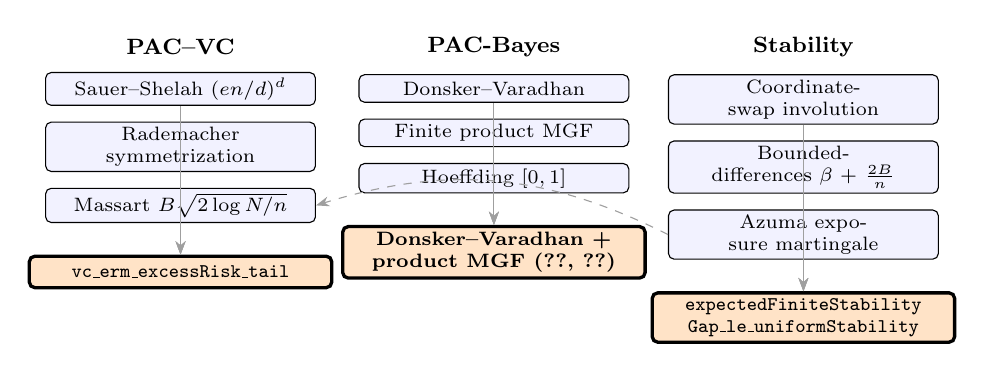
\begin{tikzpicture}[
  node distance=2mm and 4mm,
  every node/.style={font=\scriptsize},
  prim/.style={draw, rounded corners=2pt, fill=blue!5,
               inner sep=1.8pt, align=center, text width=33mm,
               minimum height=3.5mm},
  top/.style={draw, very thick, rounded corners=2pt, fill=orange!22,
              inner sep=2pt, align=center, text width=37mm,
              minimum height=4mm, font=\scriptsize\bfseries},
  hdr/.style={font=\footnotesize\bfseries},
  arr/.style={->, >=Stealth, thin, gray!75}
]
\node[hdr] (hA) {PAC--VC};
\node[hdr, right=22mm of hA] (hB) {PAC-Bayes};
\node[hdr, right=22mm of hB] (hC) {Stability};
\node[prim, below=1mm of hA] (ss)    {Sauer--Shelah $(en/d)^d$};
\node[prim, below=of ss]     (sym)   {Rademacher symmetrization};
\node[prim, below=of sym]    (mass)  {Massart $B\sqrt{2\log N/n}$};
\node[prim, below=1mm of hB] (dv)    {Donsker--Varadhan};
\node[prim, below=of dv]     (mgf)   {Finite product MGF};
\node[prim, below=of mgf]    (hoeff) {Hoeffding $[0,1]$};
\node[prim, below=1mm of hC] (swap)  {Coordinate-swap involution};
\node[prim, below=of swap]   (bd)    {Bounded-differences $\beta+\tfrac{2B}{n}$};
\node[prim, below=of bd]     (azuma) {Azuma exposure martingale};
\node[top, below=4mm of mass]  (vcerm)
  {\texttt{vc\_erm\_excessRisk\_tail}};
\node[top, below=4mm of hoeff] (mca)
  {Donsker--Varadhan +\\product MGF (\Cref{lst:dv}, \ref{lst:product-mgf})};
\node[top, below=4mm of azuma] (stab)
  {\texttt{expectedFiniteStability}\\\texttt{Gap\_le\_uniformStability}};
\draw[arr] (ss)    -- (vcerm);
\draw[arr] (sym)   -- (vcerm);
\draw[arr] (mass)  -- (vcerm);
\draw[arr] (dv)    -- (mca);
\draw[arr] (mgf)   -- (mca);
\draw[arr] (hoeff) -- (mca);
\draw[arr] (swap)  -- (stab);
\draw[arr] (bd)    -- (stab);
\draw[arr] (azuma) -- (stab);
\draw[arr, dashed] (azuma.west) to[bend right=22] (mass.east);
\end{tikzpicture}
\caption{Theorem dependency graph for the FormalSLT spine. Blue boxes
are primitives proved inside the library; orange boxes are the named
public theorems whose Lean signatures appear in
\Cref{lst:vcerm,lst:dv,lst:product-mgf,lst:stab-bounded-diff,lst:stab-expected}.
The dashed arrow marks the cross-track reuse of the Azuma
exposure-martingale tail.}
\Description{Three vertical proof chains. The PAC-VC chain stacks
Sauer-Shelah, Rademacher symmetrization, and Massart, all feeding
into the named public theorem vc\_erm\_excessRisk\_tail. The
PAC-Bayes chain stacks Donsker-Varadhan, the finite product MGF
identity, and Hoeffding for [0,1] losses, all feeding into the
Donsker-Varadhan plus product-MGF foundation. The stability chain
stacks the coordinate-swap involution, the bounded-differences
constant beta plus 2B over n, and the Azuma exposure martingale tail,
all feeding into the named public theorem
expectedFiniteStabilityGap\_le\_uniformStability. A dashed arrow
connects the Azuma node back to Massart, recording cross-track reuse
of the same exposure-martingale tail by the PAC-VC route.}
\label{fig:dep}
\end{figure*}

\subsection{The PAC-VC Spine}
\label{sec:spine}

The end-to-end finite-class spine starts with the deterministic ERM
inequality $\Risk(\hat{\imath}_S) - \Risk(i^\star)
\le 2\,\sup_i\,|\Risk(i) - \eRisk_S(i)|$ in \texttt{FormalSLT.ERM} and
ends with the VC ERM excess-risk tail. The closing theorem reads as
follows in Lean:

\begin{lstlisting}[caption={VC ERM excess-risk tail
                  (\texttt{FormalSLT/VC/SampleComplexity.lean:334}).},
                  label={lst:vcerm}]
theorem vc_erm_excessRisk_tail
    [MeasurableSpace Z] [Nonempty Z] [StandardBorelSpace Z]
    {mu : Measure Z} [IsProbabilityMeasure mu]
    {l : iota -> Z -> R} {B : R} (hB : 0 < B)
    (hl_meas : forall i, Measurable (l i))
    (hl_bdd  : forall i z, |l i z| <= B)
    {n d : N} (hn : 0 < n) (hd : 0 < d) (hdn : d <= n)
    (hGrowth_uniform : forall z : Fin n -> Z,
      (effectiveClass l z).card
        <= sum k in Finset.range (d+1), n.choose k)
    (hGrowth_neg     : forall z : Fin n -> Z,
      (effectiveClass (fun i w => -l i w) z).card
        <= sum k in Finset.range (d+1), n.choose k)
    (hhat : (Fin n -> Z) -> iota)
    (hERM : forall S, IsERM (empiricalRisk S l) (hhat S))
    (i_star : iota) {eps : R} (heps : 0 <= eps) :
    (piMeasure mu n).real
      { S | risk mu l i_star
          + 4 * B * Real.sqrt
              (2 * d * Real.log (Real.exp 1 * n / d) / n)
          + 2 * eps
        <= risk mu l (hhat S) }
      <= 2 * Real.exp (- eps^2 * n / (8 * B^2)) := by ...
\end{lstlisting}

\noindent
The inequality says that, for any class with effective-class growth
bounded by the Sauer--Shelah envelope $\sum_{k\le d} \binom{n}{k}$ and
any uniformly bounded measurable loss, an exact ERM rule
$\hat{\imath}_S$ achieves excess risk
$4B\sqrt{2 d \log(en/d)/n} + 2\varepsilon$ except on a set of
probability at most $2 \exp(-\varepsilon^{2} n / (8 B^{2}))$.

The proof chains four pieces. First, the deterministic ERM inequality
reduces excess risk to twice the uniform deviation. Second, the
\emph{Sauer--Shelah polynomial bound}
\texttt{sauerShelah\_polynomial\_bound}
(\Cref{lst:sauer-shelah}) converts the binomial-sum growth assumption to
the closed form $(en/d)^d$. Third, Massart's finite-class bound
(\texttt{Rademacher.Massart.massart\_finite\_class}) bounds the empirical
Rademacher complexity of an effective class of size $N$ by
$B\sqrt{2 \log N / n}$. Fourth, an Azuma-route generalization-gap tail
(\texttt{Azuma.GenGapTail.}\allowbreak\texttt{genGap\_tail\_bound\_azuma\_explicit})
controls the deviation of the gap from its expected value with the
sub-Gaussian exponent $\exp(-\varepsilon^2 n / (8 B^2))$. The
expectation of the gap is bounded by twice the expected Rademacher
complexity by symmetrization (the
\texttt{expected\_genGap\_le\_two}\allowbreak\texttt{\_expected\_empiricalRademacherComplexity}
theorem in \texttt{Rademacher.Symmetrization}), which combined with
Massart on the effective class produces the
$4B\sqrt{2 d \log(en/d)/n}$ deterministic threshold.

\begin{lstlisting}[caption={Sauer--Shelah polynomial bound
                  (\texttt{FormalSLT/VC/SauerShelah.lean:44}).},
                  label={lst:sauer-shelah}]
theorem sauerShelah_polynomial_bound
    {n d : N} (hd : 0 < d) (hdn : d <= n) :
    (sum k in Finset.range (d+1), (n.choose k : R))
      <= (Real.exp 1 * n / d) ^ d := by ...
\end{lstlisting}

The growth assumption $h\texttt{Growth\_uniform}$ in
\Cref{lst:vcerm} is the only place a user-supplied input enters the
combinatorial side of the spine. For binary classifiers under 0/1 loss
this assumption is discharged by the binary VC bridge:

\begin{lstlisting}[caption={Binary VC bridge: equality of effective
                  loss-pattern class and binary trace
                  (\texttt{FormalSLT/VC/BinaryVCBridge.lean:137}).},
                  label={lst:binary-vc}]
theorem effectiveClass_zeroOneLoss_card_eq_binaryClassTrace
    (h : iota -> alpha -> Bool) (x : Fin n -> alpha) :
    (effectiveClass (fun i a => zeroOneLoss (h i a) (y a))
                    (fun k => (x k, y (x k)))).card
      = (binaryClassTrace h x).card := by ...

theorem effectiveClass_zeroOneLoss_card_le_sauerShelah
    (h : iota -> alpha -> Bool) (x : Fin n -> alpha)
    {d : N} (hd : 0 < d) (hdn : d <= n)
    (hVC : forall A : Finset (Fin n),
             A.card = d -> ~ shattersOn h x A) :
    (effectiveClass _ _).card
      <= (Real.exp 1 * n / d) ^ d := by ...
\end{lstlisting}

The bridge identifies effective loss patterns with binary classification
traces, eliminating the user-supplied combinatorial growth bound from
the VC ERM tail's hypothesis list in the binary classification case.
This is the cleanest version of the standard ``patterns equal traces''
folklore that we have been able to extract.

The Rademacher-side complement to the VC route is the contraction
lemma. Working in the finite-sample sign-vector model, we prove a
\emph{comparison lemma} that lets the contraction argument step from a
real-valued Lipschitz post-composition to its empirical Rademacher
complexity by a coordinate-by-coordinate replacement, and then iterate
to the full Lipschitz contraction theorem
\texttt{empiricalRademacherComplexity\_contraction\_lipschitz} at
\texttt{FormalSLT/Rademacher/Contraction.lean:477}: for any Lipschitz
$\varphi : \R \to \R$ with constant $L$, and any finite scalar loss
class on a finite sample,
$\Rad_S(\varphi \circ F) \le L \cdot \Rad_S(F)$. The
finite-dimensional linear-predictor bound
\texttt{linearPredictor\_rademacher} at
\texttt{FormalSLT/Rademacher/LinearPredictor.lean:267} closes the
companion specialization: for $\{x \mapsto \langle w, x\rangle :
\|w\| \le R\}$ in a real inner-product space,
$\Rad_S \le R\, n^{-1}\,\sqrt{\sum_k \|x_k\|^2}$, and the
$\|x_k\| \le B$ corollary yields the textbook $RB/\sqrt{n}$ rate. The
proof goes through sign-product orthogonality, a discrete
Cauchy--Schwarz step, and an RMS bound; no contraction lemma is needed.

\subsection{PAC-Bayes Track}
\label{sec:pacbayes}

The PAC-Bayes track formalizes the change-of-measure substrate that
underlies the McAllester, Seeger, and Catoni confidence bounds. The
\texttt{FormalSLT.PACBayesKL} module defines the finite KL divergence
$\KL(\rho \,\|\, \pi) = \sum_i \rho_i \log(\rho_i / \pi_i)$ on a
finite type, proves $\KL(\rho \,\|\, \pi) \ge 0$ for any pair of
probability mass functions with full-support prior (the Gibbs
inequality), and proves the Donsker--Varadhan variational inequality:

\begin{lstlisting}[caption={Donsker--Varadhan variational inequality
                  (\texttt{FormalSLT/PACBayesKL.lean:235}).},
                  label={lst:dv}]
theorem donsker_varadhan [Nonempty iota]
    {rho pi : iota -> R}
    (hrho : IsPMF rho)
    (hpi  : IsFullSupportPMF pi)
    (f : iota -> R) :
    (sum i, rho i * f i)
      <= klDiv rho pi
       + Real.log (sum i, pi i * Real.exp (f i)) := by ...
\end{lstlisting}

The proof uses only $\log x \le x - 1$ and the Gibbs-posterior
identity; we do not import abstract Jensen / convexity machinery. The
companion module \texttt{FormalSLT.PACBayesFiniteProductMGF} lifts the
single-coordinate moment-generating function bound to the iid sample
average:

\begin{lstlisting}[caption={Finite iid product MGF factorization for
                  empirical-risk deviations
                  (\texttt{FormalSLT/PACBayesFiniteProductMGF.lean:94}).},
                  label={lst:product-mgf}]
theorem finiteProduct_mgf_empiricalRiskDeviation_eq_pow
    {n : N} [Fintype Z] (hn : 0 < n)
    (p : Z -> R) (l : iota -> Z -> R) (i : iota) (lam : R) :
    (sum S : Fin n -> Z,
        finiteProductSampleWeight p S *
          Real.exp (lam * (finitePopulationRisk p l i
                          - finiteEmpiricalRisk l i S)))
    = (sum z : Z,
        p z * Real.exp ((lam * n^(-1))
                  * (finitePopulationRisk p l i - l i z))) ^ n
\end{lstlisting}

\noindent
This is an algebraic identity on the finite product measure: the
sample-average exponential moment factors exactly as the $n$th power of
the one-coordinate moment. Combined with the prior-averaged corollary
\texttt{finitePriorAveraged\_mgf\_}\allowbreak\texttt{empiricalRiskDeviation\_le},
it provides the second ingredient of the McAllester chain. The bounded-loss
track \texttt{PACBayesBoundedLoss} closes the finite confidence surface:
a Hoeffding instantiation of the one-coordinate MGF for $[0,1]$ losses,
combined with Markov's inequality, assembles a Catoni-style fixed-$\lambda$
PAC-Bayes confidence bound and the closed good-event theorem
\texttt{pac\_bayes\_generalization}. The \texttt{PACBayesMcAllester} layer
adds fixed-budget and finite-grid McAllester-style square-root wrappers for
finite posterior classes.

We are not aware of a prior Lean 4 formalization of the core finite
PAC-Bayes change-of-measure primitives above. The Donsker--Varadhan variational inequality
in particular is, to our knowledge, the first such statement in any
proof assistant aimed specifically at PAC-Bayes use; existing Coq and
Isabelle developments cited in \Cref{sec:related} formalize Hoeffding,
Bernstein, and McDiarmid concentration but not the change-of-measure
substrate.

\subsection{Algorithmic Stability Track}
\label{sec:stability}

Algorithmic stability turns the analysis of the generalization gap from
a uniform-convergence problem into a sensitivity problem: rather than
control a supremum over hypotheses, control the change in the
algorithm's selected hypothesis when one training example is replaced.
The library defines the Bousquet--Elisseeff uniform-stability predicate
$|\ell(A(S), z) - \ell(A(S^{k\to z'}), z)| \le \beta$ as
\texttt{UniformStability} in \texttt{FormalSLT.AlgorithmicStability},
and proves the bounded-differences scaffolding for both the training
loss and the generalization gap:

\begin{lstlisting}[caption={Stability scaffolding for the training loss
                  (\texttt{FormalSLT/AlgorithmicStability.lean:464}).},
                  label={lst:stab-bounded-diff}]
theorem trainingLoss_hasBoundedDifferences
    {n : N} (hn : 0 < n)
    {A : (Fin n -> Z) -> iota} {l : iota -> Z -> R} {beta B : R}
    (hstab  : UniformStability A l beta)
    (hl_bdd : forall i z, |l i z| <= B) :
    HasBoundedDifferences (trainingLoss A l)
        (fun _ : Fin n => beta + 2 * B / n) := by ...
\end{lstlisting}

The constant $\beta + 2B/n$ decomposes as the stability contribution
$\beta$ on every term plus the $2B/n$ contribution at the
coordinate whose evaluation point changes; the symmetric statement for
the generalization gap (\texttt{stability\_genGap\_hasBoundedDifferences})
gives the $2\beta + 2B/n$ envelope. Composing with the Azuma-route
generalization-gap tail
(\texttt{hasBoundedDifferences\_tail\_azuma}) yields a high-probability
bound for stable algorithms.

The expected-gap side of the stability picture is a finite identity
proved over a finite outcome space:

\begin{lstlisting}[caption={Finite iid expected uniform-stability bound
                  (\texttt{FormalSLT/AlgorithmicStability.lean:1468}).},
                  label={lst:stab-expected},
                  basicstyle=\ttfamily\scriptsize]
theorem expectedFiniteStabilityGap_le_uniformStability_finiteProduct
    {n : N} [Fintype Z] (hn : 0 < n)
    {p : Z -> R} {A : (Fin n -> Z) -> iota}
    {l : iota -> Z -> R} {beta : R}
    (hstab : UniformStability A l beta)
    (hp_nonneg : forall z, 0 <= p z)
    (hp_sum    : sum z, p z = 1) :
    expectedFiniteStabilityGap
        (finiteProductSampleWeight p) p A l <= beta := by ...
\end{lstlisting}

\noindent
This is the finite version of the Bousquet--Elisseeff identity:
under iid finite product weights and uniform stability $\beta$, the
expected generalization gap is bounded by $\beta$. The library also includes
measure-theoretic iid product-measure wrappers under explicit integrability
assumptions, together with bounded-loss adapters that discharge those
assumptions for finite measurable hypothesis interfaces. The finite version
remains the easiest statement to audit, while the product-measure lift is the
surface used by the bounded-loss Bousquet--Elisseeff wrappers.

\section{Proof Engineering Notes}
\label{sec:engineering}

A Mathlib-supported proof-assistant project lives or dies by the
infrastructure it inherits versus the infrastructure it has to build.
Mathlib4 supplies, in usable form, the measure-theoretic foundations
(probability measures, product measures, Fubini--Tonelli, conditional
expectation, Markov's inequality), the real analysis (logarithm,
exponential, square root and their monotonicity lemmas, finite sums,
Cauchy--Schwarz on inner-product spaces), and the discrete combinatorics
(\texttt{Finset.sup'}, \texttt{Fintype}, \texttt{Finset.range},
\texttt{Nat.choose} with binomial identities). The places where we had
to build dedicated infrastructure are the empirical-process
finite-sample core, the exposure-martingale layer, and the
finite Dudley budget wrappers.

The empirical-process finite-sample core lives in
\texttt{Rademacher.FiniteSample} and \texttt{Rademacher.}\allowbreak\texttt{FiniteSampleSymmetrization}. It introduces a Boolean
sign-vector encoding, a coordinate-flip involution, a global-negation
involution, and the resulting finite combinatorial identities used in
the symmetrization step. The arithmetic is finite throughout: the
Rademacher complexity is defined as a $2^{-n}$-weighted sum over
$\texttt{Fin}\,n \to \texttt{Bool}$ rather than as an integral against a
sign measure. The product-measure envelope in
\texttt{Rademacher.Symmetrization} converts the finite-sample identity
to the integral form via
\texttt{Rademacher.ProbabilityBridge.}\allowbreak\texttt{empiricalRademacherComplexity\_eq\_integral}.
The split is a deliberate copy of Tassarotti et~al.'s deterministic /
probabilistic factoring, and it pays off: the combinatorial sign-flip
arguments live entirely in a measure-free world and the integration step
is a single bridge lemma.

The most technically intricate proof in the spine is the ghost-sample
symmetrization theorem proper (Stage 1 of
\Cref{sec:spine}), which justifies replacing
$\Risk(i) - \eRisk_S(i)$ with the decoupled gap
$\eRisk_{S'}(i) - \eRisk_S(i)$ over an iid copy $S'$. The proof requires
integrability of the generalization gap, integrability of the decoupled
gap on the product measure, a Jensen step that pulls a supremum inside
an inner integral, and a Fubini step to convert the iterated integral
into the joint integral that Stage 2 (Rademacher decoupling) consumes.
The integrability lemmas alone account for roughly 200 lines of
\texttt{GhostSample.lean}.

The exposure-martingale layer in \texttt{Azuma.*} is the
infrastructure-heaviest part of the library because every step of the
McDiarmid pipeline must be reconstructed at the level of conditional
expectation. The conditional sub-Gaussian moment-generating function
bound \texttt{exposureIncrement\_hasCondSubgaussianMGF}, the partial
integral identity
\texttt{exposureMartingale\_eq\_}\allowbreak\texttt{partialIntegral\_ae}, and the absolute
value bound \texttt{abs\_partialIntegral\_step\_le} are the three pieces
that, composed with Azuma's martingale tail in Mathlib, deliver the
generalization-gap tail. The exponent is $-\varepsilon^2 n / (8 B^2)$.
The textbook product-kernel McDiarmid bound has the sharper $-\varepsilon^2
n / (2 B^2)$ exponent. The factor-of-four gap is documented in the
project's published non-claims summary; closing it requires
\texttt{MeasureTheory.condExpKernel} infrastructure that we expect
Mathlib to land in usable form, but that we cannot rely on for the
present submission.

The finite Dudley layer in \texttt{Covering.\allowbreak{}Finite\allowbreak{}SubGaussianChaining}
is the finite analogue of the continuous entropy integral
$\int \sqrt{\log N(\varepsilon)}\,d\varepsilon$. We prove finite multiscale chaining identities, an
annulus form, an integral-budget form, prefix-envelope refinements, and a
truncated interval-integral comparison that together express the discrete
Dudley statement: a finite dyadic entropy sum is bounded by finite
covering-count budgets. The companion module \texttt{Covering.TotalBoundedDudley}
connects Mathlib's \texttt{TotallyBounded} metric-space API to the finite
chain through finite-net schedules, projected finite-net wrappers, and a
supplied-supremum boundary adapter with an explicit terminal approximation
error. We are deliberate that this is still \emph{finite} chaining: the
module documentation, the published non-claims summary, and
\Cref{sec:related} all state that we do not formalize the continuous integral
itself.

The scope statement that accompanies the artifact names the boundaries that
the current spine does not cross: the sharp McDiarmid constant, the
continuous Dudley entropy integral, an infinite-class VC theorem, and
continuous-posterior or all-real-$\lambda$ PAC-Bayes variants. Each is named
with the specific dependency that would close it: a Mathlib API, a
measurability/separability bridge to our finite chain, or a covering-number
theory beyond the discrete \texttt{Fintype} setting. The scope statement
enumerates the next theorem targets and is the section of the library
documentation we expect collaborators to read first.

\section{Conclusion and Future Work}
\label{sec:conclusion}

We have presented FormalSLT, a Lean 4 library of forty-five modules and
19,339 lines of proof that closes the standard
pedagogical PAC-VC route from empirical risk minimization to a VC ERM
excess-risk tail and an explicit closed-form sample-complexity statement,
with a Sauer--Shelah polynomial bound, a binary VC bridge, a
Ledoux--Talagrand contraction lemma, and a finite-dimensional
linear-predictor Rademacher bound, all stated as machine-checked
finite-class theorems with explicit constants. We have added a
discrete Dudley-style entropy-budget layer with total-bounded finite-net and
supplied-supremum boundary adapters, a Bousquet--Elisseeff
algorithmic-stability bounded-differences scaffold with finite and
measure-theoretic iid expected-gap wrappers, and a PAC-Bayes track comprising
the Donsker--Varadhan variational inequality, a finite iid product MGF bridge,
a Catoni-form closed good-event theorem, and finite-grid McAllester-style
wrappers. The library carries no
\texttt{sorry}, no \texttt{admit}, and no custom axioms; the public
spine reduces to the canonical $\{\texttt{propext},
\texttt{Classical.choice}, \texttt{Quot.sound}\}$ axiom set.

The immediate next theorem targets are a stability-to-PAC-Bayes bridge that
exhibits a stable algorithm as a degenerate posterior, lifting the finite-grid
PAC-Bayes wrapper to a continuous posterior class, and an infinite-class VC
theorem. Beyond that, the natural longer-horizon target is the continuous
Dudley entropy integral, which we expect to formalize as a
measurability-and-separability bridge from the existing total-bounded adapter
and finite chain to the infrastructure of Mathlib's metric-space library.
A practical co-development with the YuanheZ effort, in which we share
covering-number, Gaussian-concentration, and small-ball primitives, is
the natural shape of that step. Sharper concentration constants ---
the textbook $2B^{2}$ McDiarmid exponent in particular --- await
Mathlib's \texttt{condExpKernel} API maturing into a usable
product-kernel decomposition.

The methodological design is finite-first throughout. By keeping the
hypothesis class a \texttt{Fintype}, the sample a coordinate of a
product measure, and the supremum a finite maximum, the proof spine
stays short and auditable: every constant is explicit, every
hypothesis appears in the Lean type signature, and the
\texttt{\#print axioms} trace of every public theorem reduces to
$\{\texttt{propext},\,\texttt{Classical.choice},\,\texttt{Quot.sound}\}$.
The interface to the continuous theory is the natural composition
target with the parallel Lean efforts of \Cref{sec:related}: shared
covering-number, sub-Gaussian, and chaining primitives let the finite
spine and the continuous empirical-process layer be used as joint
dependencies in downstream developments.

\bibliographystyle{ACM-Reference-Format}
\bibliography{references}

\end{document}
